% !TeX program = xelatex
\documentclass[10pt,a4paper]{ctexart} % 设置文章类型，正文字号与纸张大小

% 页面与正文常用宏包
\usepackage[margin=2cm]{geometry} % 设置页面四周页边距
\usepackage{graphicx}             % 插入图片
\usepackage{amsmath}              % 提供cases、aligned等数学公式环境
\usepackage{amssymb}              % 提供\therefore等扩展数学符号
\usepackage{booktabs}             % 提供\toprule、\midrule、\bottomrule三线表命令
\usepackage{float}                % 提供[H]固定图片、表格位置
\usepackage{subcaption}           % 提供subfigure子图环境及子图标题
\usepackage{wrapfig}              % 提供wrapfigure图文环绕环境
\usepackage{fancyhdr}             % 自定义页眉和页脚
\usepackage{hyperref}             % 生成超链接

% 页眉页脚
\pagestyle{fancy}                  % 启用fancyhdr定义的页面样式
\fancyhf{}                         % 清空默认页眉和页脚
\fancyfoot[C]{\thepage}            % 在页脚中央显示页码
\renewcommand{\headrulewidth}{0pt} % 隐藏页眉横线
\renewcommand{\footrulewidth}{0pt} % 隐藏页脚横线

% 超链接
\hypersetup{
  colorlinks=true,                % 使用彩色文字链接，而非带边框的链接
  linkcolor=red,                 % 目录、公式及图表交叉引用的颜色
  filecolor=cyan,                 % 本地文件链接的颜色
  urlcolor=blue,                  % 网址链接的颜色
  pdftitle={用霍尔法测直流圆线圈与亥姆霍兹线圈磁场预习报告},     % 写入PDF文档属性的标题
  bookmarksnumbered=true          % PDF书签显示章节编号
}

% 定义字号命令
\newcommand{\chuhao}{\fontsize{42pt}{63pt}\selectfont}
\newcommand{\xiaochu}{\fontsize{36pt}{54pt}\selectfont}
\newcommand{\yihao}{\fontsize{26pt}{39pt}\selectfont}
\newcommand{\xiaoyi}{\fontsize{24pt}{36pt}\selectfont}
\newcommand{\erhao}{\fontsize{22pt}{33pt}\selectfont}
\newcommand{\xiaoer}{\fontsize{18pt}{27pt}\selectfont}
\newcommand{\sanhao}{\fontsize{16pt}{24pt}\selectfont}
\newcommand{\xiaosan}{\fontsize{15pt}{22.5pt}\selectfont}
\newcommand{\sihao}{\fontsize{14pt}{21pt}\selectfont}
\newcommand{\xiaosi}{\fontsize{12pt}{18pt}\selectfont}
\newcommand{\wuhao}{\fontsize{10.5pt}{15.75pt}\selectfont}
\newcommand{\xiaowu}{\fontsize{9pt}{13.5pt}\selectfont}

% 章节格式
\ctexset{
  section={
    format={\CJKfontspec[AutoFakeBold=2.5]{KaiTi}\sanhao\bfseries}, % 一级标题使用三号加粗楷体
    name={,、},                                                    % 在中文章节序号后添加顿号
    number=\chinese{section},                                      % 一级标题编号使用“一、二、三”形式
    aftername={}                                                   % 取消编号与标题文字之间的空格
  },
  subsection={
    format={\CJKfontspec[AutoFakeBold=2.5]{KaiTi}\sihao\bfseries}, % 二级标题使用四号加粗楷体
  },
  subsubsection={
    format={\CJKfontspec[AutoFakeBold=2.5]{KaiTi}\xiaosi\bfseries}, % 三级标题使用小四加粗楷体
  }
}

\begin{document}

% 封面
\thispagestyle{fancy} % 封面保留底部居中的页码
\fancyfoot[C]{\thepage}
\begin{center}
  \CJKfontspec[AutoFakeBold=2.5]{KaiTi}\bfseries % 封面中文使用楷体并人工加粗，西文同时加粗
  \vspace*{2.0cm}
  \xiaochu 
    物理实验预习报告

  \vspace{3.8cm}
  \begin{minipage}{14.0cm}
    \sanhao
    \makebox[2.6cm][l]{实验名称：}
    \underline{\makebox[11.0cm][c]{用霍尔法测直流圆线圈与亥姆霍兹线圈磁场}}\par\vspace{12pt}

    \makebox[2.6cm][l]{指导老师：}
    \underline{\makebox[11.0cm][c]{郭红丽}}\par\vspace{12pt}
  \end{minipage}

  \vspace{3.8cm}
  \begin{minipage}{10.0cm}
    \sihao
    \makebox[1.4cm][l]{班级：}
    \underline{\makebox[8.0cm][c]{}}\par\vspace{10pt}

    \makebox[1.4cm][l]{姓名：}
    \underline{\makebox[8.0cm][c]{IllusoryRain}}\par\vspace{10pt}

    \makebox[1.4cm][l]{学号：}
    \underline{\makebox[8.0cm][c]{}}
  \end{minipage}

  \vspace{1.8cm}
  \sihao
    实验日期：
    \underline{\makebox[0.7cm][c]{2026}}年
    \underline{\makebox[0.7cm][c]{9}}月
    \underline{\makebox[0.7cm][c]{30}}日
    星期\underline{\makebox[0.7cm][c]{三}}上午

  \vspace{0.7cm}
  \sihao 
    浙江大学物理实验教学中心
\end{center}

\newpage
\xiaosi\songti\mdseries % 后续正文统一使用小四不加粗的宋体

\section{预习报告（10分）}

  \subsection{实验综述（5分）}

    \subsubsection{实验背景}
    \begin{itemize}
      \item 霍尔做实验：他将附有黄铜的金箔固定，金箔两端接入电源，另两端附近放置磁体两极，将金箔与黄铜间接入电流计，使得元件两侧产生电势差。
      \item 霍尔效应：当电流垂直于外磁场并通过导体时，导体两端产生电势差。
      \item 霍尔效应器件：霍尔传感器。
    \end{itemize}

    \subsubsection{实验原理}
    霍尔效应：在$x$方向通电流$I_s$，在$z$方向加磁场$B$，则在$y$方向，即试样$P$、$S$电极两侧，就开始积聚等量异号电荷，从而产生相应的附加电场。

    \begin{wrapfigure}{r}{0.25\textwidth}
      \centering
      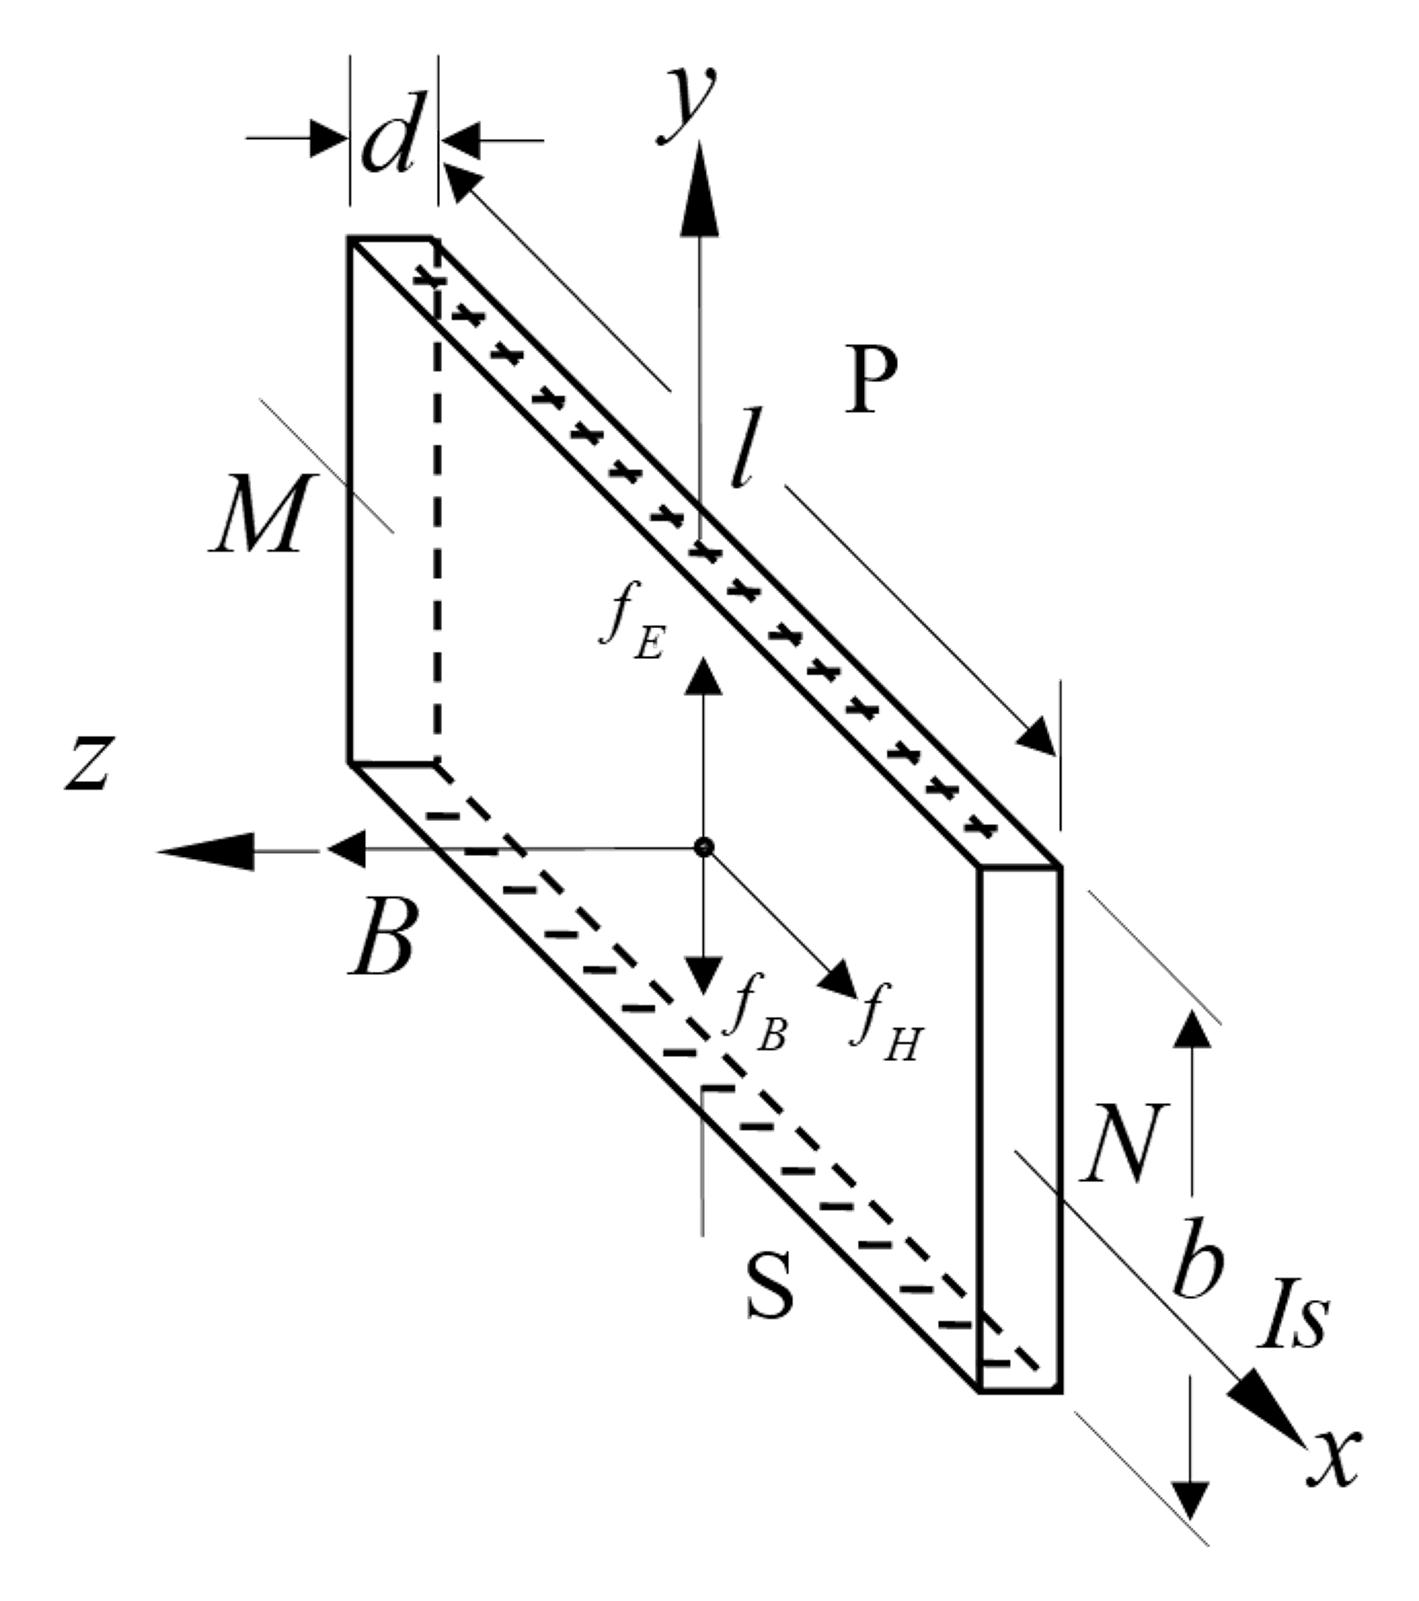
\includegraphics[width=\linewidth]{figures/图1.png}
      \caption{霍尔效应}
    \end{wrapfigure}

    磁场强度测定公式：
    电子受垂直方向磁场$B$的洛伦兹力为$f_B = evB$，电子受侧向电场$E_H$的作用力为$f_E = eE_H$。
    \[
    \begin{aligned}
        \text{稳态时}\quad
        & eE_H = evB,
          \qquad I_s = nevbd
        \\[0.8em]
        \text{所以}\quad
        & V_H = E_H b
          = \frac{1}{ne}\frac{I_s B}{d}
          = R_H \frac{I_s B}{d}
        \\[0.8em]
        \text{设}\quad
        & V_H = K_H I_s B
        \\[0.8em]
        \text{则}\quad
        & B = \frac{V_H}{K_H I_s}
    \end{aligned}
    \]

    载流圆线圈磁场分布：设半径为\(R\)、通有直流电流\(I\)的圆线圈，其轴线上距圆线圈中心\(O'\)为\(X\)处的磁感应强度为
    \[
      B
      =
      \frac{\mu_0 N_0 I R^2}
      {2\left(R^2+X^2\right)^{3/2}}
    \]
    
    其中，\(N_0\)为圆线圈的匝数，\(X\)为轴线上某一点到圆心
    \(O'\) 的距离，\(\mu_0\) 为真空磁导率，其数值为
    \[
        \mu_0 = 4\pi \times 10^{-7}\ \mathrm{H/m}
    \]
    
    载流圆线圈轴线上磁场的分布如图2所示，该磁场分布曲线是一条关于\(Y\)轴对称的单峰曲线。
    
    亥姆霍兹线圈磁场分布：亥姆霍兹线圈的特点是能在其公共轴线中点附近产生均匀磁场区域，如图3所示。

    \begin{figure}[H]
      \centering
      \begin{minipage}{0.4\textwidth}
        \centering
        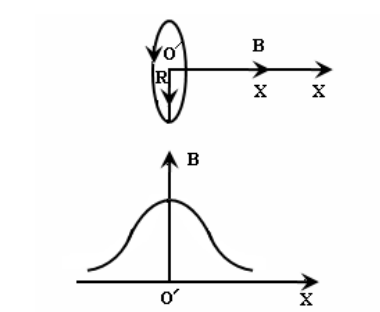
\includegraphics[width=\linewidth]{figures/图2.png}
        \caption{载流圆线圈磁场分布}
      \end{minipage}
      \hfill
      \begin{minipage}{0.4\textwidth}
        \centering
        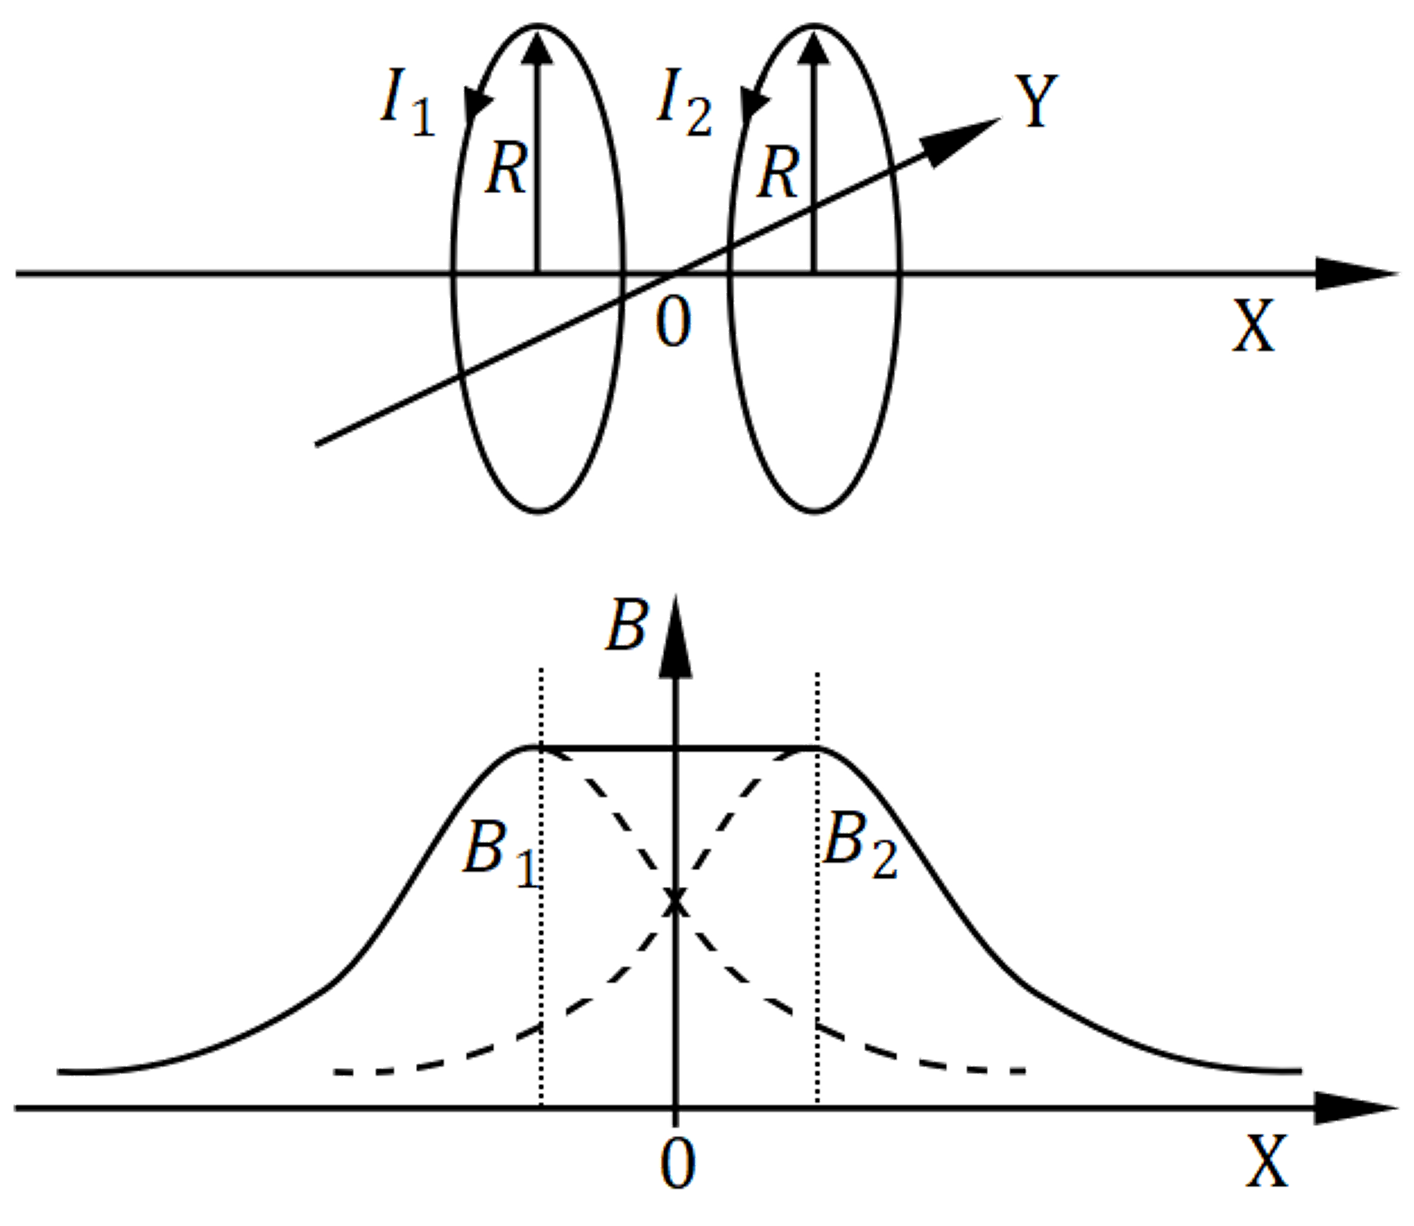
\includegraphics[width=\linewidth]{figures/图3.png}
        \caption{亥姆霍兹线圈磁场分布}
      \end{minipage}
    \end{figure}

  \subsection{实验重点（3分）}
  \begin{enumerate}
    \item 了解霍尔效应基本原理和工作特性；
    \item 测定亥姆霍兹线圈磁场分布；
    \item 掌握磁场测量方法。
  \end{enumerate}
  
  \subsection{实验难点（2分）}
  \begin{enumerate}
    \item 准确定位霍尔探头，使其敏感面垂直于磁场方向；
    \item 保持励磁电流与霍尔工作电流稳定，减小零点漂移和读数误差；
    \item 准确控制测点位置与间距，测量并比较圆线圈与亥姆霍兹线圈的磁场分布。
  \end{enumerate}

\vspace*{\fill} % 使下面内容在页面底部显示
\noindent
\begin{minipage}{\textwidth}
  注意事项：

  \begingroup
    \setlength{\leftskip}{2em} % 1--4整体向右缩进两个汉字宽度
    1. 用PDF格式上传“实验报告”，文件名：学生姓名+学号+实验名称+周次。

    2. “实验报告”必须递交在“学在浙大”本课程内对应实验项目的“作业”模块内。

    3. “实验报告”成绩必须在“浙江大学物理实验教学中心网站”-“选课系统”内查询。

    4. 教学评价必须在“浙江大学物理实验教学中心网站”-“选课系统”内进行，学生必须进行教学评价，才能看到实验报告成绩，教学评价须在本次实验结束之后3天内进行。\par
  \endgroup

  \begin{center}
    {\CJKfontspec[AutoFakeBold=2.5]{SimSun}\bfseries 浙江大学物理实验教学中心制}
  \end{center}
\end{minipage}

\end{document}
